
\subsection{Vision}

Die langfristige Vision, die \emph{Flewnit} begleitet, ist die Entwicklung eines interaktiven Paddel-Spiels unter Verwendung dieser Unified Engine mit ausgefeilter Fluid-Mechanik und -Visualisierung, partikelbasierten Rigid Bodies und Dreiecks-Mesh als Repräsentation für statische Kollisions-Geometrie. Spiele, in der große Mengen Fluid, die komplexer simuliert sind als durch Height-Fields,
%kei zeit zum referenz rauskramen ffuu ;(
%\footnote{s. Kapitel \ref{sec:relatedWork} für mehr Informationen zu Height-Field-basierter Fluidsimulation}
einen integrativen Bestandteil der Spielmechanik ausmachen, sind mir nicht bekannt.\\
Von Dreiecks-Geoemetrie wird sich eine genauere Repräsentation zur Kollisionsbehandlung erhofft, bei gleichzeitiger Ersparnis vieler Partikel, die sonst z.T große Oberflächen repäsentieren müssten. Ferner könnte die Dreiecks-Struktur später zur Simulation nicht-partikelbasierter Rigid Bodies verwendet werden.



\subsection{Paradigmen}
\label{sec:paradigm}

Vor dem Entwurf eines komplexen Softwaresystems mit einigen Zügen, die in etablierten Systemen keine so große Bedeutung haben, hat es Sinn, sich einige Paradigmen zu überlegen, welchen das System nach Möglichkeit folgen soll, um eine gewisse Konsitenz zu gewährleisten:
	
\begin{itemize}
	\item Es wurde beim Entwurf der Unified Engine für jede Simulationsdomäne eine möglichst ähnliche Struktur von Klassen 	
	und ihren Beziehungen zueinander angestrebt. Diese Ähnlichkeit spiegelt sich nach Möglichkeit in einer gemeinsamen 	
	(häufig abstrakten) Oberklasse eines jeden Konzeptes wider, wie z.B.:
	\begin{itemize}
		\item dem Simulations-Objekt als solchem
		\item der Geometrie
		\item dem Material
		\item der Szenen-Repräsentation
	\end{itemize}
	Auf diese Weise soll eine maximale \emph{Symmetrie} zwischen den Domänen hergestellt werden, so dass domänen-bedingte 
	Spezial-Behandlung von Objekten und Workflows minimiert wird.

	\item Es sollte eine Art Pipeline-Architektur entstehen, in der bestimmte Pipeline-Stages bestimmte 
	Simulations-(Zwischen)-Ergebnisse produzieren, und ggfs. anderen Stages diese zur Verfügung stellen. 
	Jede Simulationsdomäne hat ihre eigene Pipeline. Dennoch können Interdependenzen bestehen.\\
	Diesen Interdependenzen wird durch eine Konzept-spezifische Verwaltung anhand von verschiedenen 
	Singleton-Manager-Klassen nachgekommen. 
	Ein und dasselbe Objekt kann von verschiedenen Managern in unterschiedlichem Zusammenhang verwaltet 
	werden; mehr dazu in Kapitel \ref{sec:systemArchitecture}.

	\item Es sollen langfristig so viele Features (Visualisierungstechniken und -effekte, Simulationstechniken) wie möglich 
	miteinander kombinierbar sein, sofern die Kombination nicht unsinnig ist.

	\item Es soll so viel wie möglich auf der GPU berechnet werden, um die massive Paralleltät auszunutzen, 
	und um nicht durch Buffer-Transfers, die die Aufteilung von Algorithmen in CPU- und GPU- Code meist mit sich bringen, 	
	auf den Bandbreiten- und Latenz- Flaschenhals der PCI-Express-Schnittstelle zu stoßen, über welche die GPU
	and das Host-System angeschlossen ist.
	
	
	\item Es soll immer das Potential gewahrt bleiben, dass aus dem Framework -- außerhalb des Rahmens dieser 
	Bachelorarbeit -- tatsächlich noch eine Art \emph{Unified Engine} entstehen kann. Somit sind "`schnelle Hacks"',
	also unsaubere Programmiertechniken, die mit geringstem Programmierungs-Aufwand ein bestimmtes Feature implementieren,
	überall dort unbedingt zu vermeiden, wo sie die konsistente Gesamtstruktur des Systems bedrohen.

\end{itemize}



	


\subsection{Begriffe}

Im Zuge der angestrebten Vereinheitlichung der  verschiedenen Simulationsdomänen müssen wir auch einige Begriffe verallgemeinern, welche in ihrer jahrzehntelangen Tradition in der Terminologie der Computergraphik eine spezifische Bedeutung erhalten haben.
Zur besseren Einordnung stellt Abbildung \ref{fig:classicalVsUnified} ein grobes Schema dar, welches die klassische Verwendung verschiedener Engines und die einer Unified Engine gegenüber stellt:



	\begin{figure}[ht]
		%\centering
		\def\svgwidth{\textwidth}
	    \input{classicalVsUnified.pdf_tex}
	   	%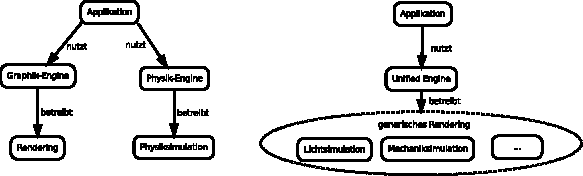
\includegraphics[width=\textwidth]{classicalVsUnified.pdf}
		\caption{Gegenüberstellung von Verwendung und Begrifflichkeiten von klassischen Engines und einer Unified Engine}
		\label{fig:classicalVsUnified}
	\end{figure}
	




\begin{description}

	\item[Rendering]
	Im Wiktionary \footnote{http://en.wiktionary.org/} wird das Verb \emph{to render} u.a. umschrieben als:
	\begin{quote}
		"`(transitive, computer graphics) To transform digital information in the form received from a repository into a 
		display on a computer screen, or for other presentation to the user."'
	\end{quote}	
	Es geht also um die Transformation einer formalen Beschreibung in eine für einen menschlichen Benutzer wahrnehmbare 
	Form. Diese muss entgegen der gewöhnlichen Verwendung des Begriffes nicht zwingend visueller, sondern kann z.B. auch 
	akustischer oder haptischer Natur sein, übertragen durch Lautsprecher oder Force-Feedback-Devices.\\
	
	Verallgemeinern wir den Begriff \emph{Rendering} weiter, gemäß der Übersetzung der Verb-Form als 
	\emph{erbringen}, \emph{machen} \footnote{http://www.dict.cc/?s=render},	
	und in Anlehnung an seine Ethymologie (Quelle: Wiktionary),
	\begin{quote}
		"`From Old French \emph{rendre} (“to render, to make”)"' [...]
	\end{quote}
	
	bietet sich eine freie Übersetzung als \emph{Erzeugung eines Zustandes beliebiger Natur} an.\\
	Unter diese generische (Um)-Deutung des Begriffes fällt nun auch \emph{die Ausführung beliebig gearteter Simulation}.
	
	Zur besseren Abgrenzung kann man von \emph{generischem Rendering} und dem klassischen 
	\emph{visuellen Rendering} sprechen. Dies soll im weiteren Verlauf dieser Arbeit der Fall sein.\\
	Eine \emph{Unified Engine} (s.u.) betreibt also \emph{generisches Rendering}.
	
	
	\item[Unified Engine] Alternativ-Bezeichnung: \emph{Unified Rendering Engine};
	eine \emph{Unified Engine} betreibt \emph{generisches Rendering}, indem sie bestimmte Aspekte einer 
	\emph{Welt}\footnote{Diese Welt muss dabei nicht zwingend unserer Realität ähneln oder entsprechen.} simuliert. 
	Darunter kann das klassische (visuelle) Rendering fallen, aber auch die Simulation von Geräuschen und von Mechanik, und 
	beliebige weitere Domänen. Die Domänen sollen dabei durch Abstraktion gemeinsamer Eigenschaften so ähnlich wie möglich
	organisiert sein.
	
	\item[Simulation] Das Begriffspaar \emph{Rendering} und \emph{Physiksimulation} ist im Kontext dieser versuchten 
	Vereinheitlichung nicht mehr angemessen. Stattdessen sollten wir den Simulations-Gedanken aufgreifen und anstelle von
	\emph{Rendering} lieber von \emph{Licht-Simulation} sprechen. Auf diese Weise werden missverständliche abwechselnde 
	Verwendungen des Begriffs \emph{Rendering} vermieden.\\
	Der Begriff der \emph{Physiksimulation} ist auch nicht ganz sauber, da streng genommen Licht auch ein physikalisches
	Phänomen ist, und somit vom Begriff eingeschlossen wird, statt sich abzugrenzen. Es bietet sich die alternative und 
	genauere  Bezeichnung \emph{Mechanik-Simulation} an. Die Quantenmechanik vor Augen (der Name spricht für sich) und 
	damit den Umstand, dass auch Photonen an mechanischen Vorgängen teilnehmen, ist zwar selbst dies keine saubere 	
	Abgrenzung, aber auf dem angestrebten Niveau einer plausiblen (im Kontrast zur "`korrekten"') Echtzeit-Simulation, 
	welche mit der Newton'schen Physik auskommen wird, ist diese Abgrenzung klar genug.
	
	\item[GPU Computing]
	Für gewöhnlich bekannt als Begriff, der GPGPU-Computing beschreibt in Abgrenzung zur Verwendung der GPU zur Berechnung 
	von	Bildern mittels Graphik-APIs, soll auch dieser Begriff im Folgenden einen Oberbegriff darstellen für beliebige
	Berechnungen, die auf der GPU ausgeführt werden, gleichgültig ob in einem GPGPU- oder einem Graphik-bezogenen Kontext.
	Die Abgrenzung der Domänen "`Graphik"' und "`General Purpose"' ist nicht zwingend anhand der benutzten APIs 
	festzustellen. So kann man z.B. mit einer GPGPU-API Ray Tracing für visuelles Rendering betreiben, oder aber 
	General Purpose-Berechnungen mit Graphik-APIs anstellen.
	\footnote{Vor der Zeit der \emph{Compute Unified Device Architecture (CUDA)}-Devices und der gleichnamigen GPGPU-
	Programmier-Umgebung von Nvidia, welche mit dem G80-Chipsatz bzw. der GeForce 8800 GTX 2006 ihren Anfang nahm, war
	der "`Missbrauch"' von Graphik-APIs für den Endbenutzer die einzige Möglichkeit, die massive Rechenleistung der
	Graphikkarte für generische Zwecke zu nutzen.}
	
	Da im Computer jede Operation eine Form von Berechnung darstellt, erscheint die Verwendung von \emph{GPU Computing}
	als Oberbegriff legitim. GPU Computing unterteilt sich dann in \emph{Graphik-Programmierung} (für gewöhnlich, aber 
	nicht zwingend durch Verwendung von Graphik-APIs wie OpenGL oder Direct3D) und \emph{GPGPU} (für gewöhnlich, aber 
	nicht zwingend durch Verwendung von GPGPU-APIs wie CUDA, DirectCompute oder OpenCL).
		
	%don't know yet if it makes sense here to define the below words
	%\item[Material] 
	%\item[Buffer] 

	
\end{description}

Somit ist die erste Symmetrie zwischen den Simulationsdomänen durch eine Anpassung der Terminologie bewerkstelligt.





\subsection{Schwerpunkte}

Die Entwicklung eines solchen \emph{Unified Frameworks}
\footnote{Von einer \emph{Engine} soll im Kontext der Implementierung im Rahmen dieser Bachelorarbeit noch nicht 
gesprochen werden, da dieser Begriff eine viel zu große Vollständigkeit der Implementation suggeriert.} umfasst sehr viele Aspekte, und einige werden wohl in dieser Ausarbeitung keine Erwähnung finden. Um die didaktischen Ziele von Seite \pageref{list:didacticGoals} nicht aus den Augen zu verlieren, wurden folgende Schwerpunkte gesetzt:

\begin{description}

	\item[Entwicklungs-Umgebung]
	Nach Anfängen unter Windows 7 und Visual Studio 2010 gab es bald Probleme beim Compilen von Dependencies auf 
	64 Bit. Es wurde dann zu Ubuntu Linux\footnote{http://www.ubuntu.com/} und Eclipse\footnote{http://www.eclipse.org/} 
	in Kombination mit dem Cross-Platform Build-System CMake\footnote{http://www.cmake.org/} gewechselt. 
	Es war ein großes Anliegen, ein System zu entwickeln, welches vollständig für die 64 Bit-Prozessor-Architektur
	kompiliert ist, da viele Register der heutigen 64Bit-Prozessoren sonst ungenutzt bleiben.
	Das Paket-Management der Linux-basierten Betriebsysteme und die konsequente Implementierung fast aller Programme in 64 
	Bit erleichtern das Einrichten der Dependencies ungemein. Schon alleine dafür hat sich der Umstieg 
	gelohnt.
	\footnote{Einen sehr sehr großen Dank möchte ich an dieser Stelle Lubosz Sarnecki aussprechen, der mich mit 
	meiner zuvor sehr eingeschränkten Linux-Erfahrung unermüdlich mit Profi-Support bei der fortgeschrittenen Customization 
	des Betriebsystems versorgt hat. Ohne ihn wäre mir dieser schnelle, weitgehend reibungslose Umstieg nicht gelungen.}
	Für die Source Code-Versionsverwaltung kam \emph{Git}\footnote{http://git-scm.com/} zum Einsatz.\\
	Dieser Punkt ist hier genannt, da eine nicht unerhebliche Umgewöhnung durch den Wechsel aus der gewohnten
	Entwicklungs-Umgebung (Windows, Visual Studio, GLUT, SVN) nötig war, somit auch hierfür Zeit eingeplant werden musste.

	\item[Dependencies]
	\label{focus:dependencies}
	Das Endziel einer potenten, modernen Engine sollte auf keinen Fall durch die Wahl suboptimaler Bibliotheken 
	eingeschränkt werden. Andererseits sollten, um Compile- und Link-Zeiten gering zu halten und Konflikte zwischen 
	Bibliotheken zu vermeiden, die Dependencies nicht zu komplex sein. Vor allem die Wahl des OpenGL-Toolkits
	\footnote{welches für die Erstellung eines Fensters mit OpenGL-Kontext verantwortlich ist}, der Input-
	Bibliothek und der Mathematik-Bibliothek musste deshalb mit Bedacht getroffen werden. Mehr dazu in Kapitel 
	\ref{sec:dependencies}.
	
	
	
	\item[Nutzung moderner OpenGL-Features]
	Mit OpenGL Version 3 erfuhr die offene Graphik-API eine gründliche Reinigung: Viele nicht mehr zeitgemäße Features 
	wurden für deprecated erklärt und durch einige neue, meist generischere Features ersetzt.
	Das Resultat ist eine schlankere API mit mehr Verantwortung für den Programmierer über die Rendering-Pipeline.
	Man muss mehr "`selbst machen", hat aber auch mehr Gestaltungsmöglichkeit.\\
	Diese Neuerung spielt dem Konzept einer Unified Engine geradezu in die Hände, da nun fast die gesamte vordefinierte 
	Semantik wie 
	\lstinline[language=GLSL]|gl_FrontMaterial.shininess,  gl_LightSource[i].diffuse, gl_NormalMatrix| oder 
	\lstinline[language=GLSL]|gl_MultiTexCoord2|
 	entfernt wurde, und man jetzt fast alle benötigten Werte entweder als generische Vertex-Attributes übergibt oder 
 	selber explizit als Uniform - Variablen definiert und setzt. Diese neue "`Freiheit der Semantik"' war eine große 
 	Inspiration, den Gedanken einer Unified Engine zu fassen, wo es nun keinen Anlass mehr gab, OpenGL-State-Variablen 
 	implizit um zu interpretieren, um bestimmte Effekte zu realisieren (Beispiel: Shadow-Map-Lookup-Matrix in eine der 	
 	Textur-Matrizen laden).
	
	Es sollte mindestens ein OpenGL Kontext im Core Profile der Version 3.3 benutzt werden. Das Core Profile stellt sicher,
	dass Routinen und Flags, die in der Spezifikation als deprecated gekennzeichnet sind, einen Fehler produzieren.
	Auf diese Weise wird die Programmierung mit nur der "`modernen"' Untermenge der OpenGL-API forciert.
	Optional sollte ein OpenGL 4 - Kontext erstellt werden können, sofern unterstützende Hardware existiert und dies vom 
	Benutzer erwünscht ist.
	Wo es sinnvoll und angebracht ist, sollten moderne Features von OpenGL verwendet werden.
	Mehr dazu in Kapitel \ref{sec:usedOpenGLfeatures}.

	
	\item[Template-Engine]
	Da GLSL\footnote{OpenGL Shading Language} und OpenCL C, die verwendeten Sprachen, 
	mit denen die GPU programmiert werden kann, nicht objekt-orientiert sind, 
	(zumindest OpenGL 3 und OpenCL 1.0) keine Mechanismen zum Überladen von Funktionen 
	haben, und noch nicht einmal eine \lstinline[language=C]|#include|-Direktive existiert,
	tendieren diese GPU-Programme, die sich einen erheblichen Anteil an ihrem Code untereinander teilen, 
	zur Code-Vervielfachung in den einzelnen Quelldateien.
	Dies schränkt die Wartbarkeit und bequeme Änderbarkeit und zuweilen auch die Lesbarkeit enorm ein.\\
	Abhilfe schafft hierbei die Nutzung einer String-Template-Engine namens \emph{Grantlee}\footnote{www.grantlee.org/}.
	Mit ihrer Hilfe lassen sich zur Laufzeit in Abhängigkeit von aktuellen Parametern angepasste GPU-Programme generieren,
	die nur den aktuell nötigen Code enthalten.
	Somit sind die generierten Programme lesbarer als wenn man sie über klassische bedingte Komplilierung 
	(mit \lstinline[language=C]|#ifdef FEATURE_XY| ... \lstinline[language=C]|#endif|-Direktiven ) geschrieben hätte.
	Weitere Erläuterungen sind auf Seite \pageref{sec:archtitectured:dependencies:Grentlee} zu finden.

	
	\item[Implementation und Kombination gängiger visueller Effekte]
	Um den softwaretechnischen Unterbau schließlich langsam seiner Verwendung zu zu führen,
	wurden einige visuelle Effekte unter Nutzung von OpenGL3/4 implementiert.
	Dank der Template-Engine lassen sich alle Effekte -- sofern sinnvoll -- zur Laufzeit in beliebiger Kombination 
	hinzu- oder abschalten.
	Die Effekte werden in Kapitel \ref{sec:genericVisualEffects} detaillierter vorgestellt.
	

	\item[Buffer-Abstraktion]
	\label{overview:bufferAbstraction}
	Der zentrale Dreh- und Angelpunkt der Unified Engine ist der \emph{Buffer}.\\
	Ist "`Buffer"' für gewöhnlich die Bezeichnung eines allokierten Speicherbereiches zur Nutzung durch ein Programm,
	verkompliziert sich diese simple Sicht auf einen Buffer durch die GPU Computing- APIs, erstens, weil man zwischen
	Host- und Device- Memory unterscheiden muss, zweitens, weil die GPU Computing- APIs den Buffern verschiedene Semantiken
	zuschreiben (generischer Buffer, Vertex Attribute Buffer, Vertex Index Buffer, Uniform Buffer, 
	Transform Feedback Buffer, Texture Buffer, Render Buffer, verschiedene Texturtypen etc.), 
	die je nach API zwischen den einzelnen Verwendungs-Kontexten (Host, OpenGL, OpenCL) 
	kompatibel zueinander sind oder auch nicht
	\footnote{Mit CUDA ist es z.B ohne weiteres möglich, einen beliebigen GPU-Buffer an eine Textur-Einheit zu binden und 	
	entsprechend wie eine Textur zu samplen. OpenCL erlaubt dies nicht. Hier muss man sich im Vorfeld 
	entscheiden, ob man einen "`normalen"' Buffer oder eine Textur haben will.}.
	Die einzelnen Buffertypen haben trotz ihrer semantischen Unterschiede und verschiedensten zugehörigen API-Routinen
	einige konzeptionelle Gemeinsamkeiten:\\
	Die meisten Buffertypen haben irgendeine Form von folgenden assoziierten Operationen:
	\begin{itemize}
		\item Allokation von Speicher
		\item Freigabe von Speicher
		\item Schreiben
		\item Lesen
		\item Kopieren
		\item Mappen von Device-Memory zu Host-Memory
		\item Spezifikation von Semantik (insb. bei OpenGL Buffers)
		\item Spezifikation von internen Datentypen, ggfs. Channel-Layout etc.
		\item Synchronisieren vor dem nächsten Zugriff
		\item Acquirering für einen Kontext zur Nutzung von API- Interoperabilität	
	\end{itemize}
	Ebenfalls ist eine Menge Meta-Information vielen Buffertypen gemeinsam:
	\begin{itemize}
		\item Name
		\item Buffergröße
		\item Buffertyp
		\item Buffer-Semantik
		\item interne Datentypen
		\item weitere Buffertyp-spezifische Meta-Informationen
		\item Information der beteiligten Kontexte ( z.B. nur Host Memory, reiner OpenGL-Buffer, 
				CL/GL-interop-Buffer mit oder ohne assoziierten Host Memory etc.)
	\end{itemize}
	
	Je nach Buffertyp und assoziierter API unterscheiden sich die Routinen, um diese Operationen auszuführen bzw. diese 	
	Meta-Informationen auszulesen, 
	%\footnote{sofern dies überhaupt möglich ist. Z.B. Host- und OpenCL Buffer brauchen für 
	%ihre Benutzung nicht zwingend definiertes Channel-Layout und Datentypen}	
	teilweise erheblich.
	Um dem Benutzer der Unified Engine die Bürde der API-spezifischen Operationen abzunehmen, und möglichst viel
	Meta-Information geschlossen zur Verfügung zu stellen, bietet sich an,
	ein vereinheitlichtes Interface bereit zu stellen, von dem konkrete Buffertypen abgeleitet werden können,
	die die entsprechenden Operationen implementieren.
	Hieraus entstanden eine Reihe von Buffer- und Texturklassen, welche zugehörige Meta-Informationen \linebreak enthalten.
	Eine detaillierte Beschreibung findet sich in Abschnitt \ref{sec:architecture:BufferAbstraction}.
	
%ersetzlos gestichen wegen doppelmoppling:	
%	\item[Performance durch Implementierung auf der GPU mit modernen GPU-Computing-APIs]	
%	auf die massive parallelität eingehen, die sowohl von visualler wie mechanischer domäne genutzt werden kann.
%	Performance-Schwerpunkt, Optimierung, auch hardware-abhängige, erwähnen, Gegenüberstellung zu alten OpenGL-nutzenden 	
%	GPUPU- Verfahren, die nicht scattern konnten in texturen rendern mussten und auch sonst etliche Nachteile hinnehmen 	
%	mussten
	
	
	\item[Effiziente Verwendung von OpenCL]
		Bei der OpenCL-Implementierung lag der Schwerpunkt sowohl bei der algorithmischen Effizienz
		als auch bei hardwarespezifischen Optimierungen. Es werden Parameter wie z.B. die Größe
		des lokalen Speichers einer OpenCL Compute Unit abgefragt, und in Verbund mit den benutzerdefinierten
		Simulations-Parametern die Konstanten im OpenCL-Code mit der 
		Template Engine und Workload-Parameter und Buffergrößen auf Seiten der Applikation entsprechend gesetzt.
		Für Details sei auf \ref{sec:hardwareOptimizations} verwiesen.



\end{description}
	
	
\clearpage
